\documentclass[a0paper,portrait]{baposter}


\usepackage{wrapfig}
\usepackage{lmodern}
\usepackage{xcolor}

\usepackage[utf8]{inputenc} %unicode support
\usepackage[T1]{fontenc}


\selectcolormodel{cmyk}

\graphicspath{{figures/}} % Directory in which figures are stored


\newcommand{\compresslist}{%
\setlength{\itemsep}{0pt}%
\setlength{\parskip}{1pt}%
\setlength{\parsep}{0pt}%
}

\newenvironment{boenumerate}
  {\begin{enumerate}\renewcommand\labelenumi{\textbf\theenumi.}}
  {\end{enumerate}}

\usepackage{amsmath}
\usepackage{palatino}
\usepackage{mathpazo}
\usepackage{fontawesome}
\usepackage{hyperref}

\newcommand{\mail}		[1]{\faEnvelope \quad {#1}}
\newcommand{\github}	[1]{\faGithub \quad {#1}}


\begin{document}


\definecolor{Black}{RGB}{0,0,0}
\definecolor{White}{RGB}{255,255,255}

% Basic colors
\definecolor{SeaGreen}{RGB}{111,189,165}
\definecolor{Cyan}{RGB}{0,166,214}
\definecolor{DarkBlue}{RGB}{34,70,122}
\definecolor{Purple}{RGB}{36,46,131}
\definecolor{Turquoise}{RGB}{50,154,179}
\definecolor{SkyBlue}{RGB}{130,187,206}

% Accent colors
\definecolor{Lavender}{RGB}{121,150,180}
\definecolor{Orange}{RGB}{216,130,62}
\definecolor{WarmPurple}{RGB}{110,50,122}
\definecolor{Fuchsia}{RGB}{178,72,146}
\definecolor{BrightGreen}{RGB}{183,200,34}
\definecolor{Yellow}{RGB}{247,234,151}
\definecolor{Pink}{RGB}{138,75,129}
\definecolor{Purple}{RGB}{69,48,117}

\definecolor{customBlockColor}{RGB}{111,189,165}
\definecolor{customAlertColor}{RGB}{31,112,173}
\newcommand{\mR}{\mathbb{R}}
\begin{poster}
{
grid=false,
headerborder=open, % Adds a border around the header of content boxes
colspacing=1em, % Column spacing
bgColorOne=white, % Background color for the gradient on the left side of the poster
bgColorTwo=white, % Background color for the gradient on the right side of the poster
borderColor=WarmPurple, % Border color
headerColorOne=Pink, % Background color for the header in the content boxes (left side)
headerColorTwo=Pink, % Background color for the header in the content boxes (right side)
headerFontColor=white, % Text color for the header text in the content boxes
boxColorOne=white, % Background color of the content boxes
textborder=rounded, %rectangle, % Format of the border around content boxes, can be: none, bars, coils, triangles, rectangle, rounded, roundedsmall, roundedright or faded
eyecatcher=false, % Set to false for ignoring the left logo in the title and move the title left
headerheight=0.11\textheight, % Height of the header
headershape=rounded, % Specify the rounded corner in the content box headers, can be: rectangle, small-rounded, roundedright, roundedleft or rounded
headershade=plain,
headerfont=\Large\textsf, % Large, bold and sans serif font in the headers of content boxes
textfont=\textsf, % Uncomment for paragraph indentation
linewidth=2pt % Width of the border lines around content boxes
}
{}
%
%---------------------------------------------------------------------------
%	TITLE AND AUTHOR NAME
%---------------------------------------------------------------------------
%
{
\color{WarmPurple}\textsf %Sans Serif
{Learning from Functions with Semi-Parametric Kernel Ridge}
} 
%
{\sf\vspace{0.5em}\\
O. Taylan Turan*, David M.J. Tax*, and Marco Loog*
\vspace{0.1em}\\
\small{Pattern Recognition Laboratory, Delft University of Technology, Van Mourik Broekmanweg 6, Delft 2628 XE, The Netherlands
}
\large{
\vspace{0.2em}\\
 \color{WarmPurple}\mail{o.t.turan@tudelft.nl} 
\hspace{0.2em}
  \github{github.com/taylanot}}
}
%
{}

\headerbox{1. Introduction}{name=intro,column=0,row=0, span=2}
{
  \begin{itemize}
    \color{Pink} \item \color{Black} Meta-learning: leverages similar learning problems (tasks) for a specific similar data-scarce target learning problem (task).
  \color{Pink} \item AIM : Come up with a meta-learning method that is interpretable with a convex loss to optimize!
  \end{itemize}
  
}

\headerbox{3. Setup}{name=maml,column=2, span=1}
{
  \begin{equation}\label{eq:data}
  y = f_a(\mathbf{x}) + \varepsilon,
  \end{equation}
where $y\in\mR$, $\mathbf{x} \in \mR^d$, and $\varepsilon$ is taken to be standard normal.  

\color{Pink} Meta-learning tasks are determined by $p_f$!
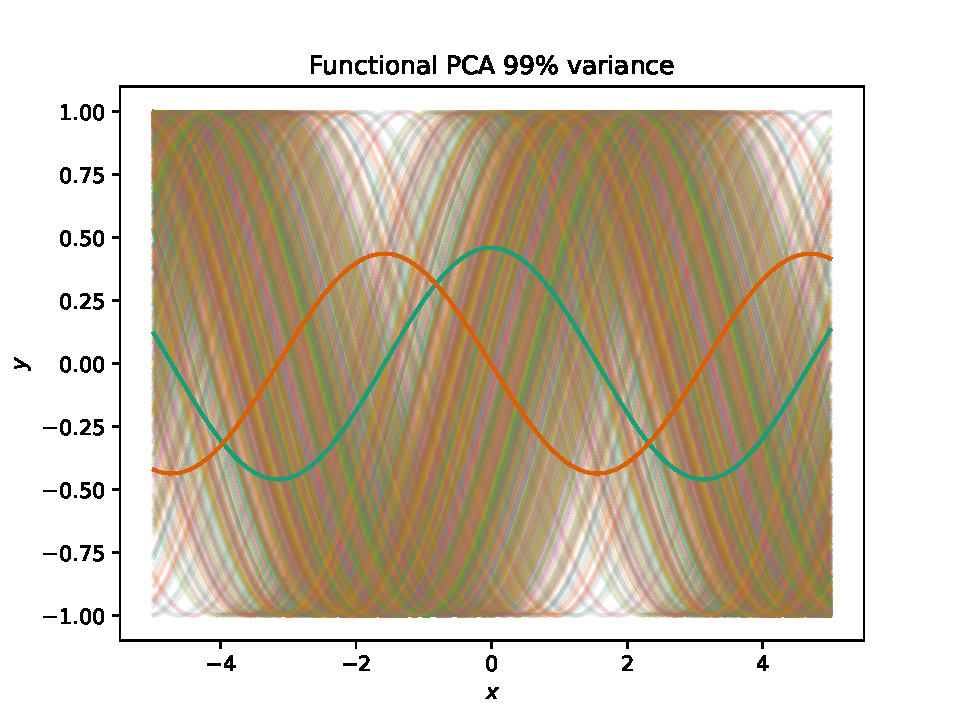
\includegraphics[width=\textwidth]{figures/illustration.pdf}
}

\headerbox{2. Semi-Parametric Kernel Ridge}{name=expr,column=0, below=intro, span=2}
{

Assuming $\tilde{f}= f + h$ where $h\in span\{\psi_p\}$ and as$\{\psi_p\}_{p=1}^M$ are real-valued functions and if the loss is taken as $\mathcal{L}=\sum_i^N(\tilde{f}(\mathbf{x}_i)-y_i)^2$. 
Then,
  \begin{equation}
  \hat{\tilde{f}} = \min_{\tilde{f}\in\mathcal{H}}\quad\sum_i^{N_a}(\tilde{f}(\mathbf{x}_i)-y_i)^2 + g(||f||_\mathcal{H})
  \end{equation}  
has the form $\tilde{f}(\cdot)=\sum^N_i\alpha_i k(\cdot,\mathbf{x}_i)+\sum_j^M\beta_j\psi_j(\cdot).$ (Semi-Parametric Representer Theorem!)

}

\headerbox{3. Open Questions}{name=q,column=2, span=1, below=maml}
{
  \begin{itemize}
    \item Regularization of $\beta$ 
    \item Can we just improve our kernels with $\{\psi_i\}_{i=1}^N$
    \item Functional PCA utilization!
  \end{itemize}
}

\headerbox{2. Semi-Parametric Kernel Ridge}{name=expr,column=0, below=intro, span=2}
{

Assuming $\tilde{f}= f + h$ where $h\in span\{\psi_p\}$ and as$\{\psi_p\}_{p=1}^M$ are real-valued functions and if the loss is taken as $\mathcal{L}=\sum_i^N(\tilde{f}(\mathbf{x}_i)-y_i)^2$. 
Then,
  \begin{equation}
  \hat{\tilde{f}} = \min_{\tilde{f}\in\mathcal{H}}\quad\sum_i^{N_a}(\tilde{f}(\mathbf{x}_i)-y_i)^2 + g(||f||_\mathcal{H})
  \end{equation}  
has the form $\tilde{f}(\cdot)=\sum^N_i\alpha_i k(\cdot,\mathbf{x}_i)+\sum_j^M\beta_j\psi_j(\cdot).$ (Semi-Parametric Representer Theorem!)


}

\headerbox{4. Synthetic Problem
}{name=res,column=0, below=expr, span=2}
{

Let us assume we are trying to solve a problem  for a 1-dimensional regression problem (D=1),
\begin{equation}
  y = \text{sin}(\mathbf{x}+\phi_{a})+\varepsilon, 
\end{equation}
where $y\in\mR$, $\mathbf{x}\in\mR^D$, $\phi_{a} \sim \mathcal{N}(\mathbf{0}, c\mathbf{I})$ and $\varepsilon\sim\mathcal{N}(0, \sigma^2)$.
  \centering
  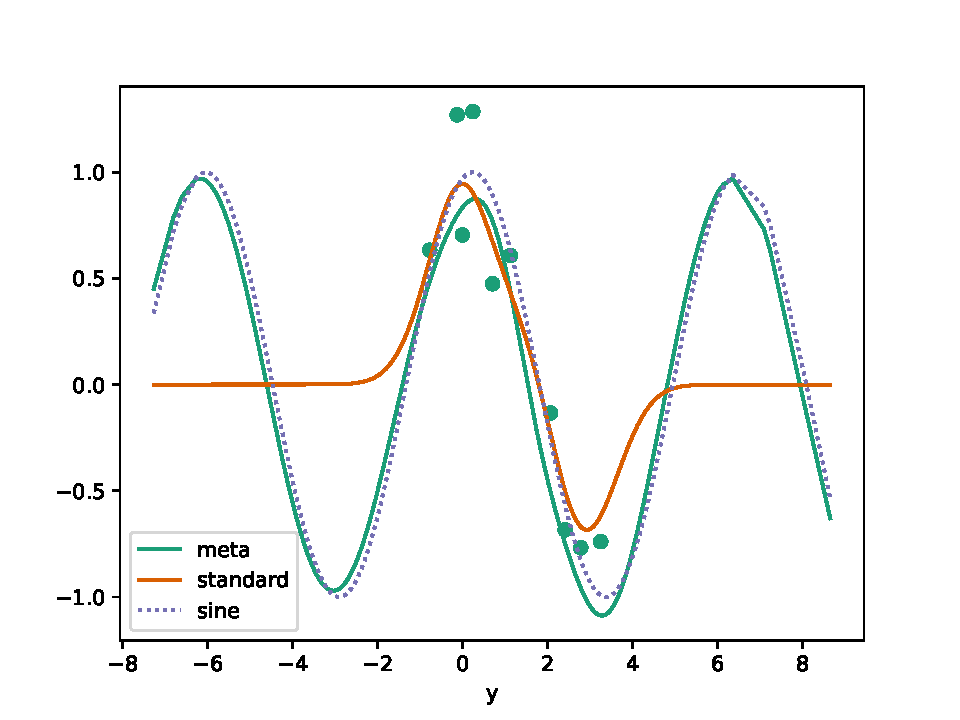
\includegraphics[width=0.5\textwidth]{figures/noise_2.pdf}

  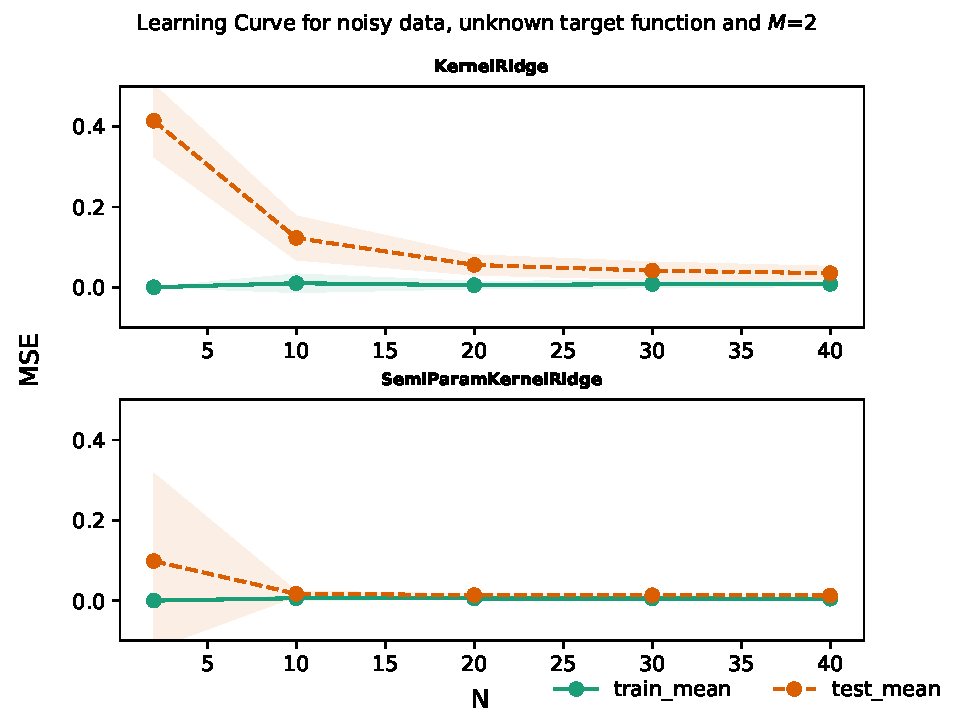
\includegraphics[width=0.45\textwidth]{figures/learningcurve2.pdf}
  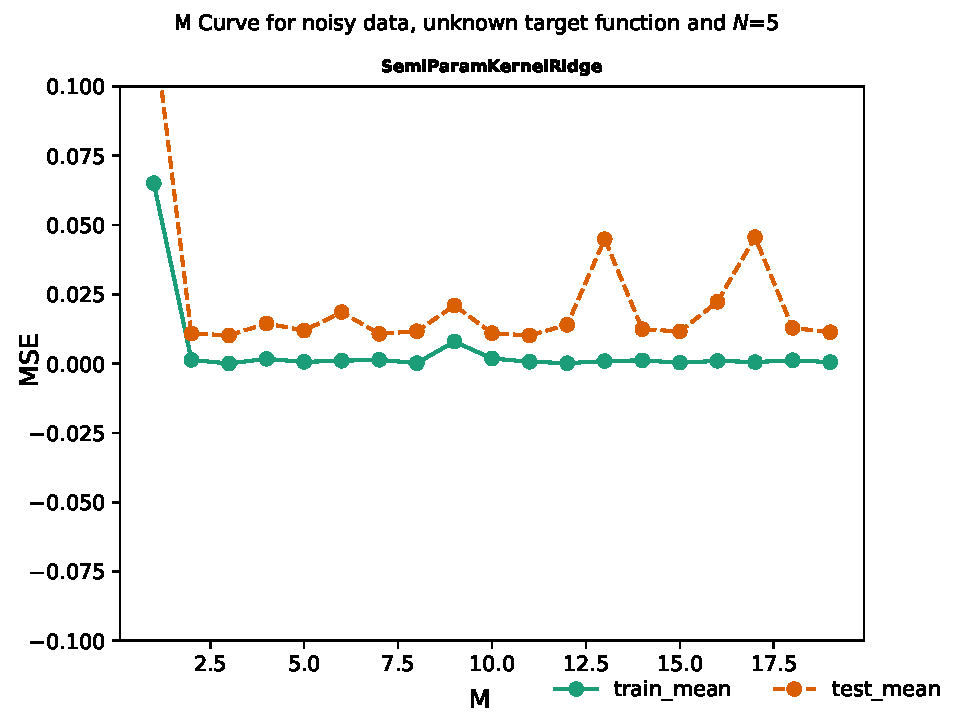
\includegraphics[width=0.45\textwidth]{figures/Mcurve5.pdf}

}

\headerbox{5.Learning Curve Application
}{name=lc,column=0, below=res, span=2}
{
  \begin{minipage}{0.5\textwidth}
    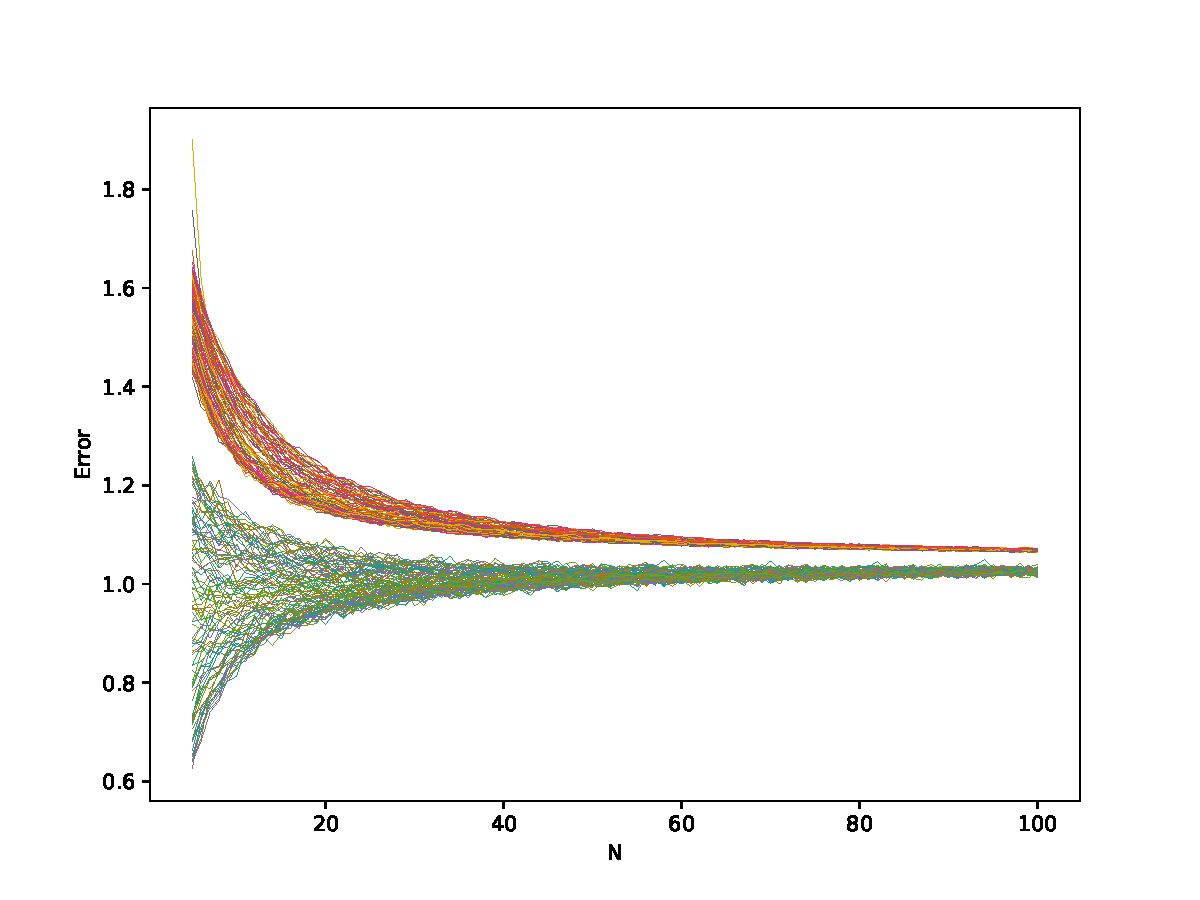
\includegraphics[width=\textwidth]{figures/lr_learning_curves.pdf}
  \end{minipage}%
  \begin{minipage}{0.5\textwidth}
    \begin{itemize}
      \item Bunch of learning curves for varying regularization $\lambda$
      \item Work in progress!!!
    \end{itemize}
  \end{minipage}
}
%\headerbox{5. Ridge Regression Learning Curve Application  
%}{name=lc,column=0, below=res, span=1}
%{
%
%  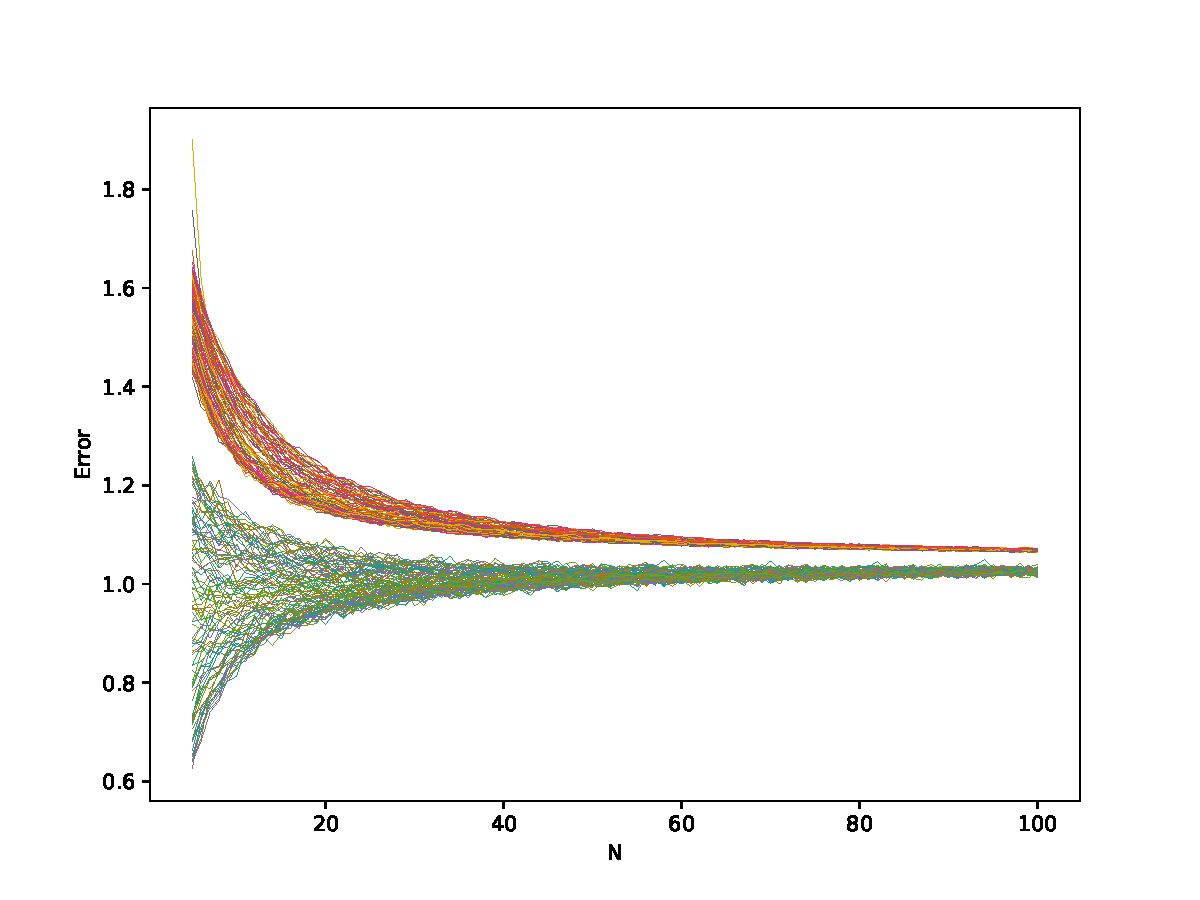
\includegraphics[width=\textwidth]{figures/lr_learning_curves.pdf}
%}
\end{poster}

\end{document}
